\documentclass[]{VUMIFTemplateClass}

\usepackage{indentfirst}
\usepackage{amsmath, amsthm, amssymb, amsfonts}
\usepackage{graphicx}
\usepackage{verbatim}
\usepackage[hidelinks]{hyperref}
\usepackage{color,algorithm,algorithmic}
\usepackage[nottoc]{tocbibind}
\usepackage{tocloft}
\usepackage{caption}
\usepackage{longtable}
\usepackage{booktabs}
\usepackage{tabularx}
\usepackage{adjustbox}
\usepackage{tikz}
\usetikzlibrary{arrows.meta, positioning, calc}

\usepackage{titlesec}
\newcommand{\sectionbreak}{\clearpage}

\makeatletter
\renewcommand{\fnum@algorithm}{\thealgorithm}
\makeatother
\renewcommand\thealgorithm{\arabic{algorithm} algoritmas}

% Lentelių stulpelis, kuriame tekstas lygiuojamas pagal kairę
\newcolumntype{L}{>{\raggedright\arraybackslash}X}

% Sekų diagramų stiliai
\tikzset{
    actor/.style={draw, rounded corners, fill=gray!10, minimum width=3.2cm,
        minimum height=1cm, align=center, font=\small\bfseries},
    lifeline/.style={dashed, gray},
    msg/.style={-{Stealth[length=2.5mm]}, thick},
    ret/.style={-{Stealth[length=2.5mm]}, thick, dashed},
    lbl/.style={font=\footnotesize, align=center, fill=white, inner sep=1.5pt},
    note/.style={draw, fill=yellow!15, font=\footnotesize, align=left,
        inner sep=3pt},
}

\bibliography{bibliografija}

\studijuprograma{Informacinių sistemų inžinerijos}
\darbotipas{Laboratorinis darbas}
\darbopavadinimas{Daugiafaktorinis autentifikavimas: OAuth 2.0 (OpenID Connect) MFA implementavimo planas}
\darbopavadinimasantras{Multi-Factor Authentication: OAuth 2.0 (OpenID Connect) Implementation Plan}
\autorius{Tomas Petronis}

\vadovas{Rolandas Gricius}

\begin{document}
\selectlanguage{lithuanian}

\onehalfspacing
\begin{titlepage}
\vskip 20pt
\begin{center}

\includegraphics[scale=0.55]{images/MIF.png}
\end{center}

\makeatletter

\vskip 20pt
\centerline{\bf \large \textbf{VILNIAUS UNIVERSITETAS}}
\vskip 10pt
\centerline{\large \textbf{MATEMATIKOS IR INFORMATIKOS FAKULTETAS}}
\vskip 10pt
\centerline{\large \textbf{\MakeUppercase{\@studijuprograma \space studijų programa}}}

\vskip 80pt
\centerline{\Large \@darbotipas}
\vskip 20pt
\begin{center}
    {\bf \LARGE \@darbopavadinimas}
\end{center}
\begin{center}
    {\bf \Large \@darbopavadinimasantras}
\end{center}
\vskip 80pt

\centering{\Large \@autorius}
\@ifundefined{@antrasautorius}{}
{
\vskip 10pt
\centering{\Large \@antrasautorius}
}
\vskip 20pt

\centering{
    \begin{tabular}{rp{.7\textwidth}}
        {\Large Darbo vadovas:} & {\Large \@vadovas}\\[10pt]
        \@ifundefined{@moksliniskonsultantas}{}
            {
                {\Large Mokslinis konsultantas:} & {\Large \@moksliniskonsultantas}\\[10pt]
            }
        \@ifundefined{@recenzentas}{}
            {
                {\Large Recenzentas:} & {\Large \@recenzentas}\\[10pt]
            }
    \end{tabular}}

\vskip 110pt

\centerline{\large \textbf{Vilnius}}
\centerline{\large \textbf{\the\year{}}}

\makeatother

\newpage
\end{titlepage}
%\newgeometry{top=2cm,bottom=2cm,right=2cm,left=3cm}
\setcounter{page}{2}

\tableofcontents
\onehalfspacing

\section{Užduoties tikslas}
\label{sec:uzduoties_tikslas}

Užduoties tikslas -- sudaryti vieno pasirinkto daugiafaktorinio autentifikavimo (\textit{angl. multi-factor authentication}, MFA) metodo implementavimo planą~\cite{VMA}. Pasirinktas metodas -- \textbf{OAuth 2.0} protokolas kartu su jo tapatybės sluoksniu \textbf{OpenID Connect} (OIDC). Antrasis faktorius -- išorinio tapatybės teikėjo (\textit{angl. identity provider}, IdP) \textit{Google} paskyra.

Plane nagrinėjama interneto aplikacija (serveris -- Node.js su TypeScript), kurioje:
\begin{itemize}
    \item \textbf{pirmasis faktorius} -- aplikacijos slaptažodis (tai, ką vartotojas žino);
    \item \textbf{antrasis faktorius} -- prisijungimas prie iš anksto susietos \textit{Google} paskyros per OAuth 2.0 ir OpenID Connect (tai, ką vartotojas turi).
\end{itemize}

Užduoties reikalavimai ir juos atitinkančios darbo dalys pateiktos \ref{tab:reikalavimai} lentelėje.

\begin{table}[H]
    \centering
    \caption{Užduoties reikalavimai ir juos atitinkančios darbo dalys.}
    \label{tab:reikalavimai}
    \begin{tabularx}{\textwidth}{L l}
        \toprule
        \textbf{Reikalavimas} & \textbf{Darbo dalis} \\
        \midrule
        Pasirinktas MFA metodas ir trumpas aprašymas, kaip jis veikia & \ref{sec:metodas} skyrius, \ref{fig:oidc_srautas} pav. \\
        Kaip vartotojas aktyvuos MFA metodą & \ref{sec:aktyvavimas} skyrius, \ref{fig:aktyvavimas} pav. \\
        Kaip vartotojas autentifikuosis MFA metodu & \ref{sec:autentifikavimas} skyrius, \ref{fig:prisijungimas} pav. \\
        Kokie duomenys saugomi duomenų bazėje & \ref{sec:duomenu_baze} skyrius, \ref{fig:db_schema} pav. \\
        Biblioteka arba servisas, kuriuo implementuojamas MFA & \ref{sec:biblioteka} skyrius \\
        Aktualūs paveikslėliai & \ref{fig:oidc_srautas}--\ref{fig:db_schema} pav. \\
        \bottomrule
    \end{tabularx}
\end{table}

Plano tekstui ir diagramoms parengti buvo pasinaudota Claude~\cite{claude}.

\section{Pasirinktas MFA metodas ir jo veikimas}
\label{sec:metodas}

\subsection{OAuth 2.0 ir OpenID Connect}
\label{subsec:oauth_oidc}

\textbf{OAuth 2.0}~\cite{rfc6749} -- tai deleguotos autorizacijos (\textit{angl. delegated authorization}) protokolas. Jis leidžia aplikacijai gauti ribotą prieigą prie vartotojo duomenų kitoje paslaugoje (pvz., \textit{Google}), nesužinant vartotojo slaptažodžio. Vartotojas prisijungia tiesiogiai prie paslaugos, o aplikacija gauna tik prieigos žetoną (\textit{angl. access token}).

Grynas OAuth 2.0 nėra autentifikavimo protokolas. Prieigos žetonas skirtas API, o ne aplikacijai, todėl iš jo aplikacija negali patikimai sužinoti, \emph{kas} ir \emph{kada} prisijungė~\cite{oauth_authentication}. Autentifikavimui naudojamas \textbf{OpenID Connect 1.0}~\cite{oidc_core} -- tapatybės sluoksnis virš OAuth 2.0. Aplikacija užklausoje nurodo \texttt{openid} sritį (\textit{angl. scope}) ir kartu su prieigos žetonu gauna \textbf{ID žetoną} (\textit{angl. ID token}). Tai tapatybės teikėjo pasirašytas JWT, aprašantis autentifikavimo įvykį. Svarbiausi jo laukai (\textit{angl. claims}):
\begin{itemize}
    \item \texttt{iss} -- žetoną išdavęs teikėjas (\textit{Google} atveju \texttt{https://accounts.google.com});
    \item \texttt{sub} -- vartotojo identifikatorius pas teikėją. Jis nekinta ir niekada nesuteikiamas kitam vartotojui~\cite{google_oidc};
    \item \texttt{aud} -- aplikacijos, kuriai skirtas žetonas, kliento identifikatorius (\texttt{client\_id});
    \item \texttt{exp}, \texttt{iat} -- žetono galiojimo pabaigos ir išdavimo laikas;
    \item \texttt{nonce} -- aplikacijos sugeneruota atsitiktinė reikšmė, susiejanti žetoną su konkrečia užklausa;
    \item \texttt{auth\_time}, \texttt{amr} -- kada ir kokiais metodais (pvz., \texttt{pwd}, \texttt{mfa}, \texttt{hwk}, \texttt{swk}) vartotojas autentifikavosi~\cite{rfc8176}. \textit{Google} šiuos laukus grąžina tik tada, kai jų paprašoma per \texttt{claims} parametrą. Be to, tai veikia tik \textit{Google} patvirtintoms (\textit{angl. verified}) produkcinėms aplikacijoms, kurių nustatymuose įjungtas \textit{security bundle}~\cite{google_security_bundle}.
\end{itemize}

Šiame plane „OAuth MFA metodas“ reiškia OAuth 2.0 autorizacijos kodo srautą su PKCE ir OpenID Connect ID žetonu, kai tapatybės teikėjas yra \textit{Google}. Protokolo dalyviai pateikti \ref{tab:roles} lentelėje.

\begin{table}[H]
    \centering
    \caption{OAuth 2.0 ir OpenID Connect dalyviai.}
    \label{tab:roles}
    \begin{tabularx}{\textwidth}{L L L}
        \toprule
        \textbf{OAuth 2.0 rolė} & \textbf{OpenID Connect rolė} & \textbf{Šiame plane} \\
        \midrule
        Išteklių savininkas (\textit{Resource Owner}) & Galutinis vartotojas (\textit{End-User}) & Vartotojas ir jo naršyklė \\
        Klientas (\textit{Client}) & Pasitikinti šalis (\textit{Relying Party}) & Mūsų aplikacija (serveris) \\
        Autorizacijos serveris (\textit{Authorization Server}) & OpenID teikėjas (\textit{OpenID Provider}) & \textit{Google} \\
        Išteklių serveris (\textit{Resource Server}) & -- & \textit{Google} API (šiame plane nenaudojamas) \\
        \bottomrule
    \end{tabularx}
\end{table}

\subsection{Kodėl tai daugiafaktorinis autentifikavimas}
\label{subsec:faktorius}

Pagal skaidrėse pateiktą autentifikavimo tipų klasifikaciją~\cite{VMA}:
\begin{itemize}
    \item \textbf{pirmasis faktorius} (aplikacijos slaptažodis) yra \emph{tai, ką vartotojas žino};
    \item \textbf{antrasis faktorius} (iš anksto susietos \textit{Google} paskyros valdymas) artimiausias tipui \emph{tai, ką vartotojas turi}. Užpuolikas gali sužinoti slaptažodį iš nutekėjusios duomenų bazės, per \textit{phishing} ataką arba todėl, kad vartotojas tą patį slaptažodį naudoja keliose sistemose. Vis tiek jis neprisijungs, jei neturi prieigos prie vartotojo \textit{Google} paskyros.
\end{itemize}

Esminė projektavimo taisyklė: grįžus iš \textit{Google}, aplikacija \emph{neieško} vartotojo pagal ID žetono \texttt{sub}. Ji \emph{palygina} \texttt{sub} su reikšme, susieta su tuo vartotoju, kuris ką tik teisingai įvedė slaptažodį. Jei vartotojas būtų ieškomas pagal \texttt{sub}, gautųsi įprastas vieno faktoriaus prisijungimas „Prisijungti su Google“, o ne MFA.

Antrojo faktoriaus stiprumas priklauso nuo to, kaip \textit{Google} autentifikuoja vartotoją. Jei \textit{Google} paskyra saugoma tik slaptažodžiu, abu faktoriai faktiškai yra žinojimo tipo (du slaptažodžiai). Todėl:
\begin{itemize}
    \item aktyvuojant MFA vartotojui rekomenduojama \textit{Google} paskyroje įjungti dviejų veiksmų patvirtinimą (\textit{angl. 2-Step Verification}, 2SV) arba \textit{passkey};
    \item produkcinėje, \textit{Google} patvirtintoje aplikacijoje galima papildomai prašyti \texttt{amr} ir \texttt{auth\_time} laukų. Tuomet priimami tik tie ID žetonai, kurių \texttt{amr} turi \texttt{mfa}, \texttt{hwk} arba \texttt{swk}, o \texttt{auth\_time} ne senesnis nei, pvz., 5 minutės~\cite{google_security_bundle,rfc8176}.
\end{itemize}

\subsection{Autorizacijos kodo srautas su PKCE}
\label{subsec:srautas}

Naudojamas autorizacijos kodo srautas (\textit{angl. Authorization Code Flow}) su PKCE (\textit{angl. Proof Key for Code Exchange})~\cite{rfc7636}. Būtent šį srautą siūlo OAuth 2.0 saugumo gerųjų praktikų dokumentas RFC~9700, o netiesioginio (\textit{angl. implicit}) srauto jame naudoti nebepatariama~\cite{rfc9700}. Srauto žingsniai (\ref{fig:oidc_srautas} pav.):
\begin{enumerate}
    \item Aplikacija sugeneruoja tris atsitiktines reikšmes -- \texttt{state}, \texttt{nonce} ir \texttt{code\_verifier} -- ir išsaugo jas serverio sesijoje. Iš \texttt{code\_verifier} apskaičiuojamas \texttt{code\_challenge} = BASE64URL(SHA-256(\texttt{code\_verifier})).
    \item Naršyklė peradresuojama į \textit{Google} autorizacijos galinį tašką (\textit{angl. authorization endpoint}) su \texttt{state}, \texttt{nonce} ir \texttt{code\_challenge}.
    \item Vartotojas prisijungia prie \textit{Google} (slaptažodis ir 2SV arba \textit{passkey}) ir patvirtina, kad sutinka pasidalinti prašomais duomenimis.
    \item \textit{Google} peradresuoja naršyklę atgal į iš anksto užregistruotą \texttt{redirect\_uri} su vienkartiniu autorizacijos kodu (\texttt{code}) ir tuo pačiu \texttt{state}.
    \item Aplikacija patikrina, ar \texttt{state} sutampa su išsaugotu sesijoje. Tada tiesioginiu TLS kanalu iškeičia kodą į žetonus \textit{Google} žetonų galiniame taške (\textit{angl. token endpoint}), pateikdama \texttt{client\_secret} ir \texttt{code\_verifier}. \textit{Google} patikrina, ar SHA-256(\texttt{code\_verifier}) sutampa su anksčiau gautu \texttt{code\_challenge}.
    \item \textit{Google} grąžina ID žetoną ir prieigos žetoną.
    \item Aplikacija patikrina ID žetono laukus \texttt{iss}, \texttt{aud}, \texttt{exp} ir \texttt{nonce}. Žetonas gautas tiesiai iš \textit{Google} per TLS, todėl OpenID Connect leidžia vietoj parašo tikrinimo pasikliauti TLS serverio patikra~\cite{oidc_core}. Vis dėlto papildomai tikrinamas ir žetono parašas pagal \textit{Google} viešuosius raktus (JWKS). Tik po visų patikrų naudojamas \texttt{sub}.
\end{enumerate}

\begin{figure}[H]
    \centering
    \begin{adjustbox}{max width=\textwidth}
    \begin{tikzpicture}
        % Dalyviai
        \node[actor] (U) at (0,0)  {Vartotojas\\(naršyklė)};
        \node[actor] (A) at (7,0)  {Aplikacija\\(serveris)};
        \node[actor] (G) at (14,0) {\textit{Google}\\(OpenID teikėjas)};

        % Gyvavimo linijos
        \foreach \x in {0,7,14} {
            \draw[lifeline] (\x,-0.5) -- (\x,-17.2);
        }

        \draw[msg] (0,-1.4) -- node[lbl, above] {1. „Prisijungti per Google“} (7,-1.4);

        \node[note] at (7,-2.5) {2. Sugeneruoja \texttt{state}, \texttt{nonce}, \texttt{code\_verifier};\\
            \texttt{code\_challenge} = BASE64URL(SHA-256(\texttt{code\_verifier}))};

        \draw[ret] (7,-4.3) -- node[lbl, above] {3. HTTP 302 peradresavimas į \textit{Google}\\
            (\texttt{state}, \texttt{nonce}, \texttt{code\_challenge}, \ldots)} (0,-4.3);

        \draw[msg] (0,-5.3) -- node[lbl, above, pos=0.25] {4. GET \texttt{/o/oauth2/v2/auth?}\ldots} (14,-5.3);

        \node[note] at (14,-6.6) {5. Prisijungimas prie \textit{Google}\\
            (slaptažodis + 2SV arba \textit{passkey})\\
            ir sutikimas (\textit{consent})};

        \draw[ret] (14,-8.5) -- node[lbl, above, pos=0.75] {6. HTTP 302 $\to$ \texttt{redirect\_uri}\\
            ?\texttt{code}=\ldots\&\texttt{state}=\ldots} (0,-8.5);

        \draw[msg] (0,-9.9) -- node[lbl, above] {7. GET \texttt{/auth/google/callback}\\
            ?\texttt{code}=\ldots\&\texttt{state}=\ldots} (7,-9.9);

        \node[note] at (7,-10.7) {8. Patikrina, ar \texttt{state} sutampa su išsaugotu sesijoje};

        \draw[msg] (7,-12.1) -- node[lbl, above] {9. POST \texttt{/token}: \texttt{code}, \texttt{client\_secret},\\
            \texttt{code\_verifier} (tiesioginis TLS kanalas)} (14,-12.1);

        \node[note] at (14,-13.0) {10. SHA-256(\texttt{code\_verifier})\\
            $\stackrel{?}{=}$ \texttt{code\_challenge}};

        \draw[ret] (14,-14.2) -- node[lbl, above] {11. \texttt{id\_token} (JWT), \texttt{access\_token}} (7,-14.2);

        \node[note] at (7,-15.3) {12. Tikrina ID žetoną: \texttt{iss}, \texttt{aud}, \texttt{exp}, \texttt{nonce},\\
            parašą (JWKS); naudoja \texttt{sub}};

        \draw[ret] (7,-16.7) -- node[lbl, above] {13. Antrasis faktorius patvirtintas} (0,-16.7);
    \end{tikzpicture}
    \end{adjustbox}
    \caption{OpenID Connect autorizacijos kodo srautas su PKCE.}
    \label{fig:oidc_srautas}
\end{figure}


Autorizacijos užklausos pavyzdys (reikšmės sutrumpintos, \texttt{code\_challenge} paimtas iš RFC~7636 pavyzdžio~\cite{rfc7636}):

\begin{verbatim}
GET https://accounts.google.com/o/oauth2/v2/auth
    ?response_type=code
    &client_id=1234567890-abc.apps.googleusercontent.com
    &redirect_uri=https://app.example.lt/auth/google/callback
    &scope=openid%20email
    &state=af0ifjsldkj
    &nonce=n-0S6_WzA2Mj
    &code_challenge=E9Melhoa2OwvFrEMTJguCHaoeK1t8URWbuGJSstw-cM
    &code_challenge_method=S256
\end{verbatim}

Iškoduotos ID žetono naudingosios dalies (\textit{angl. payload}) pavyzdys. Laukai \texttt{auth\_time} ir \texttt{amr} būna tik tada, kai jų paprašoma (žr.~\ref{subsec:oauth_oidc} poskyrį):

\begin{verbatim}
{
  "iss": "https://accounts.google.com",
  "azp": "1234567890-abc.apps.googleusercontent.com",
  "aud": "1234567890-abc.apps.googleusercontent.com",
  "sub": "110169484474386276334",
  "email": "vardenis.pavardenis@gmail.com",
  "email_verified": true,
  "nonce": "n-0S6_WzA2Mj",
  "iat": 1790412000,
  "exp": 1790415600,
  "auth_time": 1790411950,
  "amr": ["pwd", "mfa"]
}
\end{verbatim}

\subsection{Srauto apsaugos mechanizmai}
\label{subsec:apsauga}

Kiekvienas srauto parametras apsaugo nuo konkrečios atakos (\ref{tab:apsauga} lentelė). Jų praleidimas yra dažniausia OAuth implementavimo klaida~\cite{rfc9700}.

\begin{table}[H]
    \centering
    \caption{Apsaugos mechanizmai ir grėsmės, nuo kurių jie saugo.}
    \label{tab:apsauga}
    \begin{tabularx}{\textwidth}{>{\raggedright\arraybackslash}p{5cm} L}
        \toprule
        \textbf{Mechanizmas} & \textbf{Nuo ko apsaugo} \\
        \midrule
        \texttt{state} & CSRF: užpuolikas negali įpiršti savo autorizacijos atsakymo, pvz., prijungti savo \textit{Google} paskyrą prie aukos paskyros \\
        \texttt{nonce} & ID žetono pakartotinis panaudojimas (\textit{angl. replay}) ir įterpimas iš kitos sesijos \\
        PKCE (\texttt{S256}) & Autorizacijos kodo perėmimas ir įterpimas: be \texttt{code\_verifier} kodo iškeisti į žetonus negalima \\
        Tikslus \texttt{redirect\_uri} & Kodo nutekėjimas į užpuoliko adresą; \textit{Google} priima tik užregistruotus adresus \\
        \texttt{iss}, \texttt{aud}, \texttt{exp} ir parašo tikrinimas & Suklastoti, pasibaigę arba kitai aplikacijai skirti žetonai \\
        \texttt{sub}, o ne \texttt{email} & Paskyros perėmimas: el. pašto adresas gali keistis ir nebūti unikalus, o \texttt{sub} nekinta~\cite{google_oidc} \\
        HTTPS, \texttt{client\_secret} tik serveryje & Srauto perėmimas ir kliento paslapties nutekėjimas \\
        \bottomrule
    \end{tabularx}
\end{table}

\subsection{Privalumai ir trūkumai}
\label{subsec:privalumai}

\textbf{Privalumai}
\begin{enumerate}
    \item Nereikia papildomos aparatinės įrangos ar programėlės -- dauguma vartotojų jau turi \textit{Google} paskyrą.
    \item Aplikacija nesaugo jokios antrojo faktoriaus paslapties (nėra TOTP rakto ar biometrinių duomenų), tik viešą identifikatorių \texttt{sub}. Todėl duomenų bazės nutekėjimas antrojo faktoriaus neatskleidžia.
    \item Paveldimas \textit{Google} saugumas: dviejų veiksmų patvirtinimas, \textit{passkey}, įtartinų prisijungimų aptikimas.
    \item Protokolas standartizuotas~\cite{rfc6749,oidc_core}, jam yra sertifikuotų bibliotekų.
    \item Iš dalies atsparus \textit{phishing} atakoms. Kodas grąžinamas tik į užregistruotą \texttt{redirect\_uri}, o jam iškeisti reikia \texttt{client\_secret} ir \texttt{code\_verifier}. Visiškas atsparumas priklauso nuo \textit{Google} pusėje naudojamo metodo: \textit{passkey} ar saugos raktas atsparūs, SMS -- ne.
\end{enumerate}

\textbf{Trūkumai}
\begin{enumerate}
    \item Priklausomybė nuo trečiosios šalies. Sutrikus \textit{Google} paslaugai arba užblokavus vartotojo \textit{Google} paskyrą, vartotojas negalės prisijungti.
    \item Privatumas: \textit{Google} sužino, kada vartotojas jungiasi prie mūsų sistemos.
    \item Faktoriaus stiprumas priklauso nuo \textit{Google} paskyros apsaugos (žr.~\ref{subsec:faktorius} poskyrį).
    \item Jei naršyklėje jau aktyvi \textit{Google} sesija, antrasis žingsnis tampa vienu paspaudimu. Užpuolikas, turintis fizinę prieigą prie atrakinto įrenginio, jį įveiktų.
    \item Implementavimo klaidos sukuria rimtų saugumo spragų: nenaudojamas \texttt{state} ar PKCE, netinkamai tikrinamas ID žetonas, vartotojas identifikuojamas pagal \texttt{email}.
    \item Reikia \textit{Google} paskyros, interneto ryšio ir peradresavimų tarp domenų. Vartotojams be \textit{Google} paskyros reikia alternatyvaus MFA metodo.
\end{enumerate}

\section{MFA aktyvavimas}
\label{sec:aktyvavimas}

MFA gali aktyvuoti tik prisijungęs vartotojas. Aktyvavimo metu jo paskyra susiejama su \textit{Google} paskyra, t.~y. išsaugomas \textit{Google} ID žetono \texttt{sub}. Aktyvavimo seka pavaizduota \ref{fig:aktyvavimas} pav.:
\begin{enumerate}
    \item Vartotojas nustatymų skiltyje „Saugumas“ paspaudžia „Įjungti MFA per Google“.
    \item Aplikacija paprašo pakartotinai įvesti slaptažodį ir jį patikrina. Taip kitas asmuo negalės įjungti MFA pasinaudojęs palikta atvira sesija.
    \item Aplikacija sugeneruoja \texttt{state}, \texttt{nonce} ir \texttt{code\_verifier}. Jie išsaugomi serverio sesijoje kartu su tikslu \texttt{purpose = enroll} ir galiojimo laiku (10 min.).
    \item Naršyklė peradresuojama į \textit{Google} su \texttt{scope = openid email} ir \texttt{prompt = select\_account}. Taip vartotojas sąmoningai pasirenka, kurią \textit{Google} paskyrą susieti.
    \item Vartotojas prisijungia prie \textit{Google} ir sutikimo lange (\textit{angl. consent screen}) leidžia aplikacijai gauti jo identifikatorių ir el. pašto adresą.
    \item \textit{Google} grąžina vartotoją į \texttt{redirect\_uri}. Aplikacija patikrina \texttt{state}, iškeičia kodą į žetonus (su \texttt{code\_verifier}), patikrina ID žetoną ir \texttt{nonce} (žr.~\ref{subsec:srautas} poskyrį).
    \item Aplikacija patikrina, ar pora (\texttt{google}, \texttt{sub}) dar nėra susieta su kita paskyra. Jei susieta, aktyvavimas nutraukiamas.
    \item Duomenų bazėje išsaugomas susiejimas (\texttt{oauth\_identities} lentelė) ir nustatoma \texttt{users.mfa\_enabled = true}.
    \item Sugeneruojama 10 vienkartinių atkūrimo kodų. Jie parodomi vartotojui tik vieną kartą, o duomenų bazėje saugomos tik jų maišos (argon2id). Tai vienas iš skaidrėse siūlomų MFA atkūrimo būdų~\cite{VMA}.
    \item Vartotojui išsiunčiamas el. laiškas „MFA įjungtas“. Jei MFA įjungė ne jis, apie tai sužinos iš karto.
\end{enumerate}

\begin{figure}[H]
    \centering
    \begin{adjustbox}{max width=\textwidth}
    \begin{tikzpicture}
        % Dalyviai
        \node[actor] (U) at (0,0)  {Vartotojas\\(naršyklė)};
        \node[actor] (A) at (5,0)  {Aplikacija\\(serveris)};
        \node[actor] (G) at (10,0) {\textit{Google}\\(OpenID teikėjas)};
        \node[actor] (D) at (15,0) {Duomenų\\bazė};

        % Gyvavimo linijos
        \foreach \x in {0,5,10,15} {
            \draw[lifeline] (\x,-0.5) -- (\x,-21.8);
        }

        \draw[msg] (0,-1.4) -- node[lbl, above] {1. „Įjungti MFA per Google“} (5,-1.4);

        \draw[msg] (0,-2.4) -- node[lbl, above] {2. Slaptažodis (pakartotinai)} (5,-2.4);

        \draw[msg] (5,-3.4) -- node[lbl, above, pos=0.75] {2. Slaptažodžio patikra (argon2id)} (15,-3.4);

        \node[note] at (5,-4.6) {3. \texttt{state}, \texttt{nonce}, \texttt{code\_verifier} $\to$ sesija\\
            (\texttt{purpose = enroll}, galioja 10 min.)};

        \draw[ret] (5,-6.2) -- node[lbl, above] {4. HTTP 302 $\to$ \textit{Google}} (0,-6.2);

        \draw[msg] (0,-7.4) -- node[lbl, above, pos=0.25] {4. \texttt{scope=openid email},\\
            \texttt{prompt=select\_account}} (10,-7.4);

        \node[note] at (10,-8.5) {5. Prisijungimas prie \textit{Google}\\
            ir sutikimas (\textit{consent})};

        \draw[ret] (10,-10.2) -- node[lbl, above, pos=0.75] {6. HTTP 302 $\to$ \texttt{redirect\_uri}\\
            (\texttt{code}, \texttt{state})} (0,-10.2);

        \draw[msg] (0,-11.4) -- node[lbl, above] {6. GET \texttt{/auth/google/callback}} (5,-11.4);

        \draw[msg] (5,-12.6) -- node[lbl, above] {6. POST \texttt{/token} (+\texttt{code\_verifier})} (10,-12.6);

        \draw[ret] (10,-13.6) -- node[lbl, above] {6. \texttt{id\_token}} (5,-13.6);

        \node[note] at (5,-14.6) {6. Tikrina \texttt{state}, ID žetoną, \texttt{nonce}};

        \draw[msg] (5,-15.8) -- node[lbl, above, pos=0.75] {7. Ar (\texttt{google}, \texttt{sub}) jau susietas?} (15,-15.8);

        \draw[ret] (15,-16.8) -- node[lbl, above, pos=0.25] {7. Ne} (5,-16.8);

        \draw[msg] (5,-18.0) -- node[lbl, above, pos=0.75] {8. INSERT \texttt{oauth\_identities};\\
            \texttt{mfa\_enabled = true}} (15,-18.0);

        \draw[msg] (5,-19.2) -- node[lbl, above, pos=0.75] {9. INSERT 10 \texttt{code\_hash} (argon2id)} (15,-19.2);

        \draw[ret] (5,-20.2) -- node[lbl, above] {9. Atkūrimo kodai (rodomi 1 kartą)} (0,-20.2);

        \draw[msg] (5,-21.2) -- node[lbl, above] {10. El. laiškas „MFA įjungtas“} (0,-21.2);
    \end{tikzpicture}
    \end{adjustbox}
    \caption{MFA aktyvavimo seka.}
    \label{fig:aktyvavimas}
\end{figure}


MFA išjungimui ir susietos \textit{Google} paskyros pakeitimui reikalingas sėkmingas OAuth patvirtinimas (žr.~\ref{subsec:step_up} poskyrį). Kitaip užpuolikas, sužinojęs tik slaptažodį, galėtų MFA tiesiog išjungti.

\section{Autentifikavimas MFA metodu}
\label{sec:autentifikavimas}

\subsection{Prisijungimo eiga}
\label{subsec:prisijungimas}

Vartotojas, kuriam MFA aktyvuotas, prisijungia dviem žingsniais (\ref{fig:prisijungimas} pav.):
\begin{enumerate}
    \item Vartotojas įveda el. pašto adresą ir slaptažodį (pirmasis faktorius).
    \item Aplikacija patikrina slaptažodžio maišą (argon2id). Jei slaptažodis teisingas ir \texttt{mfa\_enabled = true}, sesija dar \emph{nesukuriama}. Išsaugoma tik laukiančioji būsena (\textit{angl. pending}): \texttt{pending\_user\_id}, \texttt{state}, \texttt{nonce} ir \texttt{code\_verifier}. Ji galioja 5 min.
    \item Naršyklė peradresuojama į \textit{Google}. Parametro \texttt{login\_hint} reikšmė yra susietos paskyros \texttt{sub}, todėl \textit{Google} iš karto pasiūlo teisingą paskyrą~\cite{google_oidc}.
    \item Vartotojas prisijungia prie \textit{Google}. Jei naršyklėje jau yra aktyvi \textit{Google} sesija, pakanka ją patvirtinti.
    \item \textit{Google} grąžina vartotoją į \texttt{redirect\_uri}. Aplikacija patikrina \texttt{state}, iškeičia kodą į žetonus (su \texttt{code\_verifier}), patikrina ID žetoną ir \texttt{nonce}. Tada \textbf{palyginamas ID žetono \texttt{sub} su susietu \texttt{provider\_sub}}. Produkcinėje aplikacijoje papildomai tikrinama, ar \texttt{amr} turi \texttt{mfa}, \texttt{hwk} arba \texttt{swk} ir ar \texttt{auth\_time} pakankamai naujas.
    \item \textbf{Sėkmė.} Sukuriama nauja sesija su nauju sesijos identifikatoriumi, kad būtų išvengta sesijos fiksavimo (\textit{angl. session fixation}). Atnaujinamas \texttt{last\_used\_at}, laukiančioji būsena ištrinama.
    \item \textbf{Nesėkmė} (vartotojas atšaukė prisijungimą, \texttt{sub} nesutampa, žetonas netinkamas arba baigėsi laukimo laikas). Prisijungimas atmetamas, įvykis įrašomas į \texttt{auth\_events}, bandymų skaičius ribojamas. Vartotojui išsiunčiamas pranešimas su bandymo laiku, naršykle ir vieta~\cite{VMA}, o prisijungimo lange pasiūloma naudoti atkūrimo kodą.
\end{enumerate}

\begin{figure}[H]
    \centering
    \begin{adjustbox}{max width=\textwidth}
    \begin{tikzpicture}
        % Dalyviai
        \node[actor] (U) at (0,0)  {Vartotojas\\(naršyklė)};
        \node[actor] (A) at (5,0)  {Aplikacija\\(serveris)};
        \node[actor] (G) at (10,0) {\textit{Google}\\(OpenID teikėjas)};
        \node[actor] (D) at (15,0) {Duomenų\\bazė};

        % Gyvavimo linijos
        \foreach \x in {0,5,10,15} {
            \draw[lifeline] (\x,-0.5) -- (\x,-23.0);
        }

        \draw[msg] (0,-1.4) -- node[lbl, above] {1. El. paštas + slaptažodis} (5,-1.4);

        \draw[msg] (5,-2.4) -- node[lbl, above, pos=0.75] {2. Slaptažodžio patikra (argon2id)} (15,-2.4);

        \draw[ret] (15,-3.4) -- node[lbl, above, pos=0.25] {2. \texttt{mfa\_enabled}, \texttt{provider\_sub}} (5,-3.4);

        \node[note] at (5,-4.7) {2. Slaptažodis teisingas $\to$ tik laukiančioji būsena:\\
            \texttt{pending\_user\_id}, \texttt{state}, \texttt{nonce},\\
            \texttt{code\_verifier} (galioja 5 min.)};

        \draw[ret] (5,-6.3) -- node[lbl, above] {3. HTTP 302 $\to$ \textit{Google}} (0,-6.3);

        \draw[msg] (0,-7.5) -- node[lbl, above, pos=0.25] {3. \texttt{login\_hint} = susietas \texttt{sub}} (10,-7.5);

        \node[note] at (10,-8.7) {4. Prisijungimas prie \textit{Google}\\
            (jei sesija aktyvi -- tik patvirtinimas)};

        \draw[ret] (10,-10.4) -- node[lbl, above, pos=0.75] {5. HTTP 302 $\to$ \texttt{redirect\_uri}\\
            (\texttt{code}, \texttt{state})} (0,-10.4);

        \draw[msg] (0,-11.6) -- node[lbl, above] {5. GET \texttt{/auth/google/callback}} (5,-11.6);

        \draw[msg] (5,-12.8) -- node[lbl, above] {5. POST \texttt{/token} (+\texttt{code\_verifier})} (10,-12.8);

        \draw[ret] (10,-13.8) -- node[lbl, above] {5. \texttt{id\_token}} (5,-13.8);

        \node[note] at (5,-15.1) {5. Tikrina \texttt{state}, ID žetoną, \texttt{nonce};\\
            \textbf{ar \texttt{sub} = susietas \texttt{provider\_sub}?}};

        % alt fragmentas: sėkmė arba nesėkmė
        \draw[thick] (-1.9,-16.2) rectangle (16.9,-22.6);
        \node[draw, thick, fill=white, font=\footnotesize\bfseries, anchor=north west,
            inner sep=2pt] at (-1.9,-16.2) {alt};
        \node[font=\footnotesize, fill=white, anchor=north west, inner sep=1.5pt]
            at (-1.0,-16.25) {[\texttt{sub} sutampa]};

        \draw[msg] (5,-17.3) -- node[lbl, above, pos=0.75] {6. \texttt{last\_used\_at}, \texttt{mfa\_success}} (15,-17.3);

        \draw[ret] (5,-18.3) -- node[lbl, above] {6. Nauja sesija (naujas ID)} (0,-18.3);

        \draw[dashed] (-1.9,-18.9) -- (16.9,-18.9);
        \node[font=\footnotesize, fill=white, anchor=north west, inner sep=1.5pt]
            at (-1.8,-18.95) {[\texttt{sub} nesutampa / atšaukta / klaida]};

        \draw[msg] (5,-20.0) -- node[lbl, above, pos=0.75] {7. \texttt{auth\_events}: \texttt{mfa\_failed}} (15,-20.0);

        \draw[ret] (5,-21.0) -- node[lbl, above] {7. Prisijungimas atmestas} (0,-21.0);

        \draw[msg] (5,-22.0) -- node[lbl, above] {7. Įspėjimas el. paštu} (0,-22.0);
    \end{tikzpicture}
    \end{adjustbox}
    \caption{Prisijungimas su MFA: slaptažodis ir \textit{Google} patvirtinimas.}
    \label{fig:prisijungimas}
\end{figure}


\subsection{Kada dar reikalauti MFA}
\label{subsec:step_up}

Pagal skaidrių rekomendacijas~\cite{VMA} OAuth patvirtinimas reikalingas ne tik prisijungiant. Tas pats srautas (su \texttt{purpose = step\_up}) naudojamas ir kai vartotojas:
\begin{itemize}
    \item keičia slaptažodį arba el. pašto adresą;
    \item išjungia MFA arba keičia susietą \textit{Google} paskyrą;
    \item sesijoje gauna aukštesnes teises (pvz., administratoriaus).
\end{itemize}
Tokiems veiksmams priimamas tik neseniai atliktas patvirtinimas (pvz., per paskutines 5 min.). Be to, MFA turi būti taikomas visiems prisijungimo būdams. Pavyzdžiui, slaptažodžio atkūrimas el. paštu neturi leisti apeiti \textit{Google} žingsnio.

\subsection{Vartotojo patirties gerinimas}
\label{subsec:rizika}

Dažnas MFA reikalavimas gali erzinti vartotojus, todėl galima taikyti rizika paremtą MFA~\cite{VMA}. Sėkmingai prisijungus, įrenginiui išduodamas pasirašytas „patikimo įrenginio“ slapukas (\texttt{HttpOnly}, \texttt{Secure}, galioja 30 d.). Tada \textit{Google} žingsnio reikalaujama tik jungiantis iš naujo įrenginio ar neįprastos vietos arba po nesėkmingų bandymų.

\subsection{MFA atkūrimas}
\label{subsec:atkurimas}

Praradęs prieigą prie \textit{Google} paskyros, vartotojas negalėtų prisijungti. Todėl numatomi atkūrimo būdai~\cite{VMA}:
\begin{itemize}
    \item vienkartiniai atkūrimo kodai, gauti aktyvuojant MFA. Panaudotas kodas pažymimas, o vartotojas raginamas iš naujo susieti \textit{Google} paskyrą;
    \item galimybė susieti antrą MFA metodą (pvz., TOTP programėlę), kad vieno metodo praradimas neužrakintų paskyros;
    \item kraštutiniu atveju -- kreipimasis į klientų aptarnavimą, kuris griežtai patikrina vartotojo tapatybę.
\end{itemize}

\section{Duomenų bazė}
\label{sec:duomenu_baze}

OAuth antrajam faktoriui duomenų bazėje nereikia saugoti jokios paslapties -- pakanka susieti vartotoją su jo \textit{Google} identifikatoriumi \texttt{sub}. Siūloma schema pavaizduota \ref{fig:db_schema} pav., o lentelių laukai aprašyti \ref{tab:db_users}--\ref{tab:db_auth_events} lentelėse.

\begin{figure}[H]
    \centering
    \begin{adjustbox}{max width=\textwidth}
    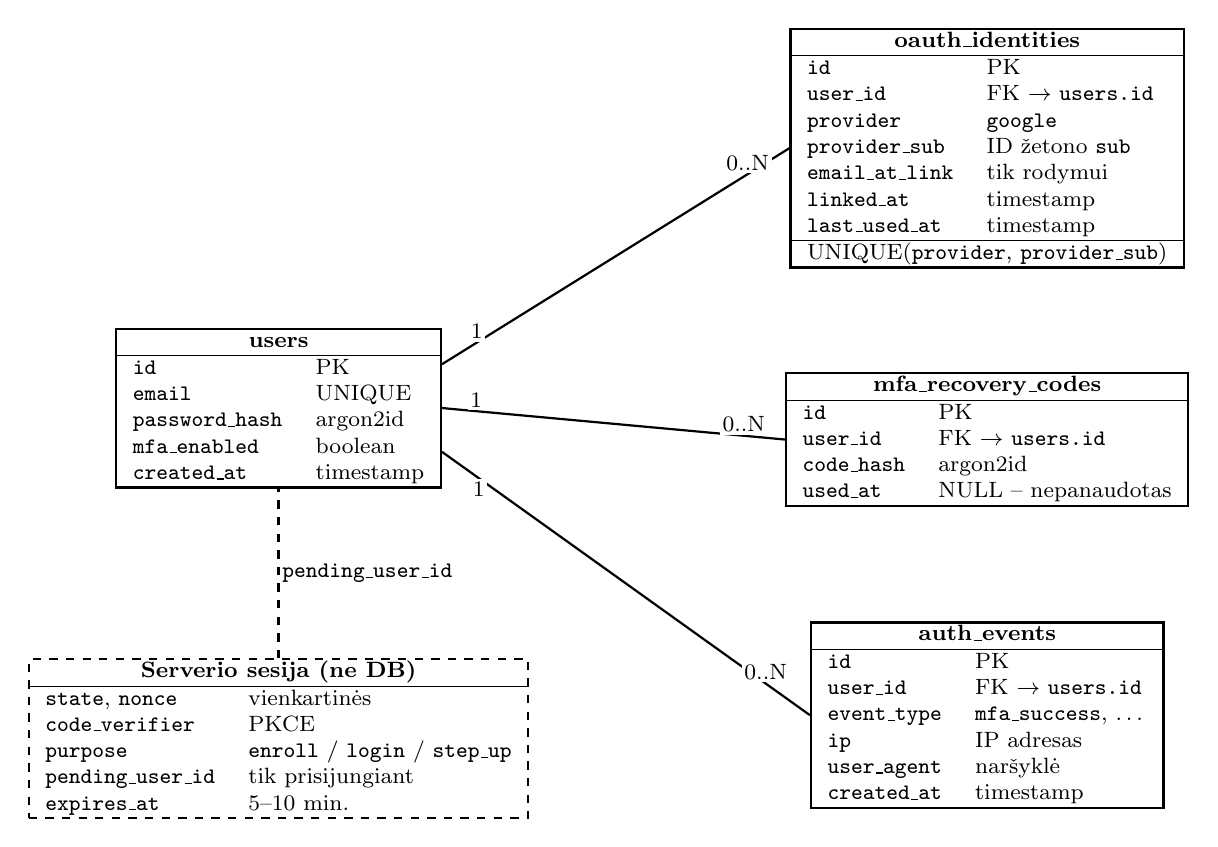
\begin{tikzpicture}[
        entity/.style={draw, thick, fill=white, inner sep=0pt, font=\footnotesize},
        session/.style={draw, thick, dashed, fill=white, inner sep=0pt, font=\footnotesize},
        rel/.style={thick},
        card/.style={font=\footnotesize, fill=white, inner sep=1pt},
    ]
        \node[entity] (users) at (0,0) {%
            \begin{tabular}{l l}
                \multicolumn{2}{c}{\textbf{users}} \\ \hline
                \texttt{id}             & PK \\
                \texttt{email}          & UNIQUE \\
                \texttt{password\_hash} & argon2id \\
                \texttt{mfa\_enabled}   & boolean \\
                \texttt{created\_at}    & timestamp \\
            \end{tabular}};

        \node[entity] (oauth) at (9,3.3) {%
            \begin{tabular}{l l}
                \multicolumn{2}{c}{\textbf{oauth\_identities}} \\ \hline
                \texttt{id}              & PK \\
                \texttt{user\_id}        & FK $\to$ \texttt{users.id} \\
                \texttt{provider}        & \texttt{google} \\
                \texttt{provider\_sub}   & ID žetono \texttt{sub} \\
                \texttt{email\_at\_link} & tik rodymui \\
                \texttt{linked\_at}      & timestamp \\
                \texttt{last\_used\_at}  & timestamp \\ \hline
                \multicolumn{2}{l}{UNIQUE(\texttt{provider}, \texttt{provider\_sub})} \\
            \end{tabular}};

        \node[entity] (codes) at (9,-0.4) {%
            \begin{tabular}{l l}
                \multicolumn{2}{c}{\textbf{mfa\_recovery\_codes}} \\ \hline
                \texttt{id}         & PK \\
                \texttt{user\_id}   & FK $\to$ \texttt{users.id} \\
                \texttt{code\_hash} & argon2id \\
                \texttt{used\_at}   & NULL -- nepanaudotas \\
            \end{tabular}};

        \node[entity] (events) at (9,-3.9) {%
            \begin{tabular}{l l}
                \multicolumn{2}{c}{\textbf{auth\_events}} \\ \hline
                \texttt{id}          & PK \\
                \texttt{user\_id}    & FK $\to$ \texttt{users.id} \\
                \texttt{event\_type} & \texttt{mfa\_success}, \ldots \\
                \texttt{ip}          & IP adresas \\
                \texttt{user\_agent} & naršyklė \\
                \texttt{created\_at} & timestamp \\
            \end{tabular}};

        \node[session] (sess) at (0,-4.2) {%
            \begin{tabular}{l l}
                \multicolumn{2}{c}{\textbf{Serverio sesija (ne DB)}} \\ \hline
                \texttt{state}, \texttt{nonce} & vienkartinės \\
                \texttt{code\_verifier}        & PKCE \\
                \texttt{purpose}               & \texttt{enroll} / \texttt{login} / \texttt{step\_up} \\
                \texttt{pending\_user\_id}     & tik prisijungiant \\
                \texttt{expires\_at}           & 5--10 min. \\
            \end{tabular}};

        \draw[rel] (users.15) -- node[card, pos=0.1, above] {1} node[card, pos=0.88, above] {0..N} (oauth.west);
        \draw[rel] (users.0) -- node[card, pos=0.1, above] {1} node[card, pos=0.88, above] {0..N} (codes.west);
        \draw[rel] (users.-15) -- node[card, pos=0.1, below] {1} node[card, pos=0.88, above] {0..N} (events.west);
        \draw[rel, dashed] (sess.north) -- node[card, right] {\texttt{pending\_user\_id}} (users.south);
    \end{tikzpicture}
    \end{adjustbox}
    \caption{Duomenų bazės schema ir laikini sesijos duomenys.}
    \label{fig:db_schema}
\end{figure}


\begin{table}[H]
    \centering
    \caption{Lentelė \texttt{users} (jau egzistuojanti, papildoma \texttt{mfa\_enabled} lauku).}
    \label{tab:db_users}
    \begin{tabularx}{\textwidth}{l l L}
        \toprule
        \textbf{Laukas} & \textbf{Tipas} & \textbf{Paskirtis} \\
        \midrule
        \texttt{id} & UUID, PK & Vartotojo identifikatorius \\
        \texttt{email} & TEXT, UNIQUE & Prisijungimo vardas \\
        \texttt{password\_hash} & TEXT & Slaptažodžio maiša (argon2id) -- pirmasis faktorius \\
        \texttt{mfa\_enabled} & BOOLEAN & Ar reikalauti antrojo faktoriaus \\
        \texttt{created\_at} & TIMESTAMP & Paskyros sukūrimo laikas \\
        \bottomrule
    \end{tabularx}
\end{table}

\begin{table}[H]
    \centering
    \caption{Lentelė \texttt{oauth\_identities} (vartotojo ir \textit{Google} paskyros susiejimas).}
    \label{tab:db_oauth}
    \begin{tabularx}{\textwidth}{l l L}
        \toprule
        \textbf{Laukas} & \textbf{Tipas} & \textbf{Paskirtis} \\
        \midrule
        \texttt{id} & UUID, PK & Įrašo identifikatorius \\
        \texttt{user\_id} & UUID, FK & Nuoroda į \texttt{users.id} \\
        \texttt{provider} & TEXT & Tapatybės teikėjas (\texttt{google}) \\
        \texttt{provider\_sub} & TEXT & ID žetono \texttt{sub}; pagal jį tikrinamas antrasis faktorius \\
        \texttt{email\_at\_link} & TEXT & \textit{Google} el. paštas susiejimo metu. Naudojamas tik rodymui, bet ne tikrinimui \\
        \texttt{linked\_at} & TIMESTAMP & Susiejimo laikas \\
        \texttt{last\_used\_at} & TIMESTAMP & Paskutinio sėkmingo patvirtinimo laikas \\
        \bottomrule
    \end{tabularx}
\end{table}

Lentelei \texttt{oauth\_identities} taikomi du unikalumo apribojimai. UNIQUE(\texttt{provider}, \texttt{provider\_sub}) užtikrina, kad viena \textit{Google} paskyra būtų susieta tik su viena mūsų sistemos paskyra. UNIQUE(\texttt{user\_id}, \texttt{provider}) leidžia vartotojui susieti tik vieną \textit{Google} paskyrą.

\begin{table}[H]
    \centering
    \caption{Lentelė \texttt{mfa\_recovery\_codes} (vienkartiniai atkūrimo kodai).}
    \label{tab:db_recovery}
    \begin{tabularx}{\textwidth}{l l L}
        \toprule
        \textbf{Laukas} & \textbf{Tipas} & \textbf{Paskirtis} \\
        \midrule
        \texttt{id} & UUID, PK & Įrašo identifikatorius \\
        \texttt{user\_id} & UUID, FK & Nuoroda į \texttt{users.id} \\
        \texttt{code\_hash} & TEXT & Atkūrimo kodo maiša (argon2id); pats kodas nesaugomas \\
        \texttt{used\_at} & TIMESTAMP, NULL & Panaudojimo laikas (NULL -- kodas dar nepanaudotas) \\
        \bottomrule
    \end{tabularx}
\end{table}

\begin{table}[H]
    \centering
    \caption{Lentelė \texttt{auth\_events} (autentifikavimo įvykių žurnalas).}
    \label{tab:db_auth_events}
    \begin{tabularx}{\textwidth}{l l L}
        \toprule
        \textbf{Laukas} & \textbf{Tipas} & \textbf{Paskirtis} \\
        \midrule
        \texttt{id} & UUID, PK & Įrašo identifikatorius \\
        \texttt{user\_id} & UUID, FK & Nuoroda į \texttt{users.id} \\
        \texttt{event\_type} & TEXT & \texttt{mfa\_enrolled}, \texttt{mfa\_success}, \texttt{mfa\_failed}, \texttt{mfa\_disabled}, \texttt{recovery\_used} \\
        \texttt{ip} & TEXT & IP adresas (vietai nurodyti pranešime vartotojui) \\
        \texttt{user\_agent} & TEXT & Naršyklė ir įrenginys \\
        \texttt{created\_at} & TIMESTAMP & Įvykio laikas \\
        \bottomrule
    \end{tabularx}
\end{table}

Jei taikomas rizika paremtas MFA (žr.~\ref{subsec:rizika} poskyrį), papildomai reikalinga lentelė \texttt{trusted\_devices}. Joje saugomi \texttt{user\_id}, slapuko maiša, naršyklė ir galiojimo pabaiga.

\textbf{Laikini duomenys (serverio sesija, ne duomenų bazė).} Vienam OAuth srautui reikalingos reikšmės saugomos serverio sesijoje:
\begin{itemize}
    \item \texttt{state}, \texttt{nonce}, \texttt{code\_verifier} -- vienkartinės atsitiktinės reikšmės;
    \item \texttt{purpose} -- srauto tikslas: \texttt{enroll}, \texttt{login} arba \texttt{step\_up};
    \item \texttt{pending\_user\_id} -- vartotojas, teisingai įvedęs slaptažodį (tik prisijungiant);
    \item \texttt{expires\_at} -- galiojimo pabaiga (5--10 min.).
\end{itemize}
Šios reikšmės ištrinamos iš karto po grįžimo iš \textit{Google}, nesvarbu, ar patvirtinimas pavyko.

\textbf{Kas nesaugoma.} Laikantis duomenų kiekio mažinimo principo~\cite{bdar}, nesaugomi:
\begin{itemize}
    \item \textit{Google} slaptažodis -- aplikacija jo niekada nemato;
    \item prieigos ir atnaujinimo (\textit{angl. refresh}) žetonai. Antrajam faktoriui jie nereikalingi, o jų saugojimas tik didintų riziką;
    \item visas ID žetonas -- pakanka jo \texttt{sub}.
\end{itemize}

\textbf{Konfigūracija.} \texttt{GOOGLE\_CLIENT\_ID}, \texttt{GOOGLE\_CLIENT\_SECRET} ir \texttt{REDIRECT\_URI} laikomi aplinkos kintamuosiuose arba slaptųjų duomenų saugykloje, ne duomenų bazėje. \texttt{client\_secret} niekada neturi patekti į naršyklę ar kodo repozitoriją.

\section{Biblioteka ir servisas}
\label{sec:biblioteka}

\subsection{Servisas -- \texorpdfstring{\textit{Google}}{Google}}
\label{subsec:google}

\textit{Google} atlieka OpenID teikėjo vaidmenį. Aplikacijai \textit{Google Auth Platform} (\textit{Google Cloud Console}) reikia:
\begin{itemize}
    \item sukurti OAuth kliento identifikatorių, kurio tipas „Web application“. Gaunami \texttt{client\_id} ir \texttt{client\_secret};
    \item užregistruoti leidžiamą peradresavimo adresą, pvz., \url{https://app.example.lt/auth/google/callback};
    \item sukonfigūruoti sutikimo langą su sritimis \texttt{openid} ir \texttt{email};
    \item produkcinei aplikacijai -- praeiti \textit{Google} patvirtinimą ir nustatymuose įjungti \texttt{amr} bei \texttt{auth\_time} laukus (\textit{security bundle})~\cite{google_security_bundle}.
\end{itemize}
Visus \textit{Google} galinius taškus biblioteka sužino automatiškai iš atradimo dokumento (\textit{angl. discovery document}) \url{https://accounts.google.com/.well-known/openid-configuration}~\cite{google_oidc}.

\subsection{Biblioteka -- \texorpdfstring{\texttt{openid-client}}{openid-client}}
\label{subsec:openid_client}

Implementacijai pasirinkta \texttt{openid-client}~\cite{openid_client} (6.x versija) -- OAuth 2.0 ir OpenID Connect kliento biblioteka JavaScript ir TypeScript aplinkoms (Node.js 20 ir naujesnėms). Ji pasirinkta, nes:
\begin{itemize}
    \item yra \textit{OpenID Certified} -- sertifikuota pagal Basic, FAPI 1.0 ir FAPI 2.0 \textit{Relying Party} profilius;
    \item palaiko atradimo dokumentą, autorizacijos kodo srautą su PKCE, \texttt{state} ir \texttt{nonce} tikrinimą;
    \item nėra susieta su konkrečiu teikėju, todėl vėliau galima pridėti kitą OpenID teikėją (pvz., \textit{Microsoft});
    \item parašyta TypeScript kalba ir tinka mūsų aplinkai (Node.js, TypeScript).
\end{itemize}

Srauto žingsnius atliekančios bibliotekos funkcijos pateiktos \ref{tab:biblioteka} lentelėje.

\begin{table}[H]
    \centering
    \caption{Srauto žingsniai ir juos atliekančios \texttt{openid-client} funkcijos.}
    \label{tab:biblioteka}
    \begin{tabularx}{\textwidth}{l L}
        \toprule
        \textbf{Funkcija} & \textbf{Paskirtis} \\
        \midrule
        \texttt{discovery()} & Nuskaito \textit{Google} atradimo dokumentą ir sukuria kliento konfigūraciją \\
        \texttt{randomPKCECodeVerifier()} & Sugeneruoja \texttt{code\_verifier} \\
        \texttt{calculatePKCECodeChallenge()} & Apskaičiuoja \texttt{code\_challenge} (S256) \\
        \texttt{randomState()}, \texttt{randomNonce()} & Sugeneruoja \texttt{state} ir \texttt{nonce} \\
        \texttt{buildAuthorizationUrl()} & Sudaro autorizacijos užklausos adresą \\
        \texttt{authorizationCodeGrant()} & Patikrina \texttt{state}, iškeičia kodą į žetonus su \texttt{code\_verifier}, patikrina ID žetono laukus ir \texttt{nonce} \\
        \texttt{enableNonRepudiationChecks()} & Papildomai įjungia ID žetono parašo tikrinimą pagal JWKS \\
        \texttt{tokens.claims()} & Grąžina ID žetono laukus (\texttt{sub}, \texttt{amr}, \ldots) \\
        \bottomrule
    \end{tabularx}
\end{table}

Alternatyvos -- \textit{Passport.js} strategijos, \textit{Google} biblioteka \texttt{google-auth-library} arba tapatybės valdymo platformos (\textit{Auth0}, \textit{Keycloak}). Pasirinkta \texttt{openid-client}, nes ji sertifikuota, nesusieta su konkrečiu teikėju ir nereikalauja papildomos infrastruktūros.

\sectionnonum{Išvados}
\label{sec:isvados}

Žemiau pateikiamos laboratorinio darbo išvados:
\begin{itemize}
    \item OAuth 2.0 yra autorizacijos protokolas, todėl autentifikavimui naudojamas jo OpenID Connect sluoksnis ir ID žetonas.
    \item OAuth veikia kaip antrasis faktorius tik tada, kai grįžus iš \textit{Google} ID žetono \texttt{sub} \emph{palyginamas} su jau slaptažodžiu autentifikuoto vartotojo susieta reikšme, o ne naudojamas vartotojui surasti.
    \item Saugiam įgyvendinimui būtini \texttt{state}, \texttt{nonce}, PKCE, tikslus \texttt{redirect\_uri} ir kruopštus ID žetono tikrinimas. Visa tai atlieka sertifikuota \texttt{openid-client} biblioteka.
    \item Duomenų bazėje pakanka saugoti \textit{Google} \texttt{sub}, atkūrimo kodų maišas ir autentifikavimo įvykius -- jokios antrojo faktoriaus paslapties saugoti nereikia.
    \item Metodo stiprumas priklauso nuo \textit{Google} paskyros apsaugos. Todėl rekomenduojama reikalauti \textit{Google} dviejų veiksmų patvirtinimo ir numatyti atkūrimo kodus bei alternatyvų MFA metodą.
\end{itemize}


\singlespacing

\printbibliography[title = {Šaltiniai}]
\end{document}
